\documentclass[class=minimal, border = 0pt, crop]{standalone}
\usepackage{pgf}
\usepackage{tkz-euclide}
\usepackage[utf8]{inputenc}
\usepackage{amsmath}
\usepackage{amsthm}
\DeclareMathAlphabet\mathbb{U}{msb}{m}{n}
%==========================================
\usetikzlibrary{arrows}
\usetikzlibrary{automata}
\usetikzlibrary{shapes}
\usetikzlibrary{calc}
\usetikzlibrary{backgrounds}
\usetikzlibrary{decorations.pathreplacing}
\usetikzlibrary{positioning}
%==========================================
\pagestyle{empty}
\begin{document}
\centering
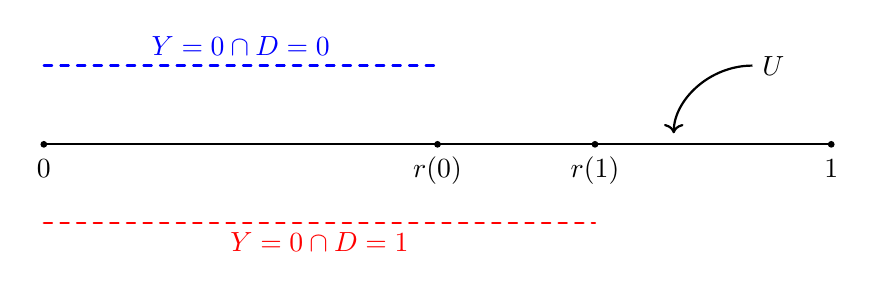
\begin{tikzpicture}
% \coordinate (O) at (0,0);
%  \draw[->] (0,0) -- (10,0) coordinate[label = {right:$\mathbb{E}[Y(0)]$}] (xmax);
%  \draw[->] (0,0) -- (0,10) coordinate[label = {above:$\mathbb{E}[Y(1)]$}] (ymax);
%  \draw[->,help lines] (0,0) -- (9.3,9.3);
%  \draw[help lines] (6.15,6.15) -- (5.95,6.35) -- (6.15,6.55) -- (6.35,6.35);
%  \draw[help lines] (0,0)+(0:1.2) arc(0:45:1.2) ;
%  \draw[fill=red!50] (1.3,4.9) rectangle (4.2,7.1);
%  \draw[fill=blue!50] (1.5,5) rectangle (4,7);
%  \draw[help lines] (6.15,6.15) -- (3,9.3);
%  \draw[color=red, dashed] (0,5.8) -- (3.25,9.05);
%  \draw[color=red, dashed] (0,0.7) -- (5.8,6.5);
%  \draw[color=blue, dashed] (0,5.5) -- (3.4,8.9);
%  \draw[color=blue, dashed] (0,1) -- (5.65,6.65);
%  \draw[color=blue] (0,1) -- (0,5.5);
%  \draw[color=red] (0,0.7) -- (0,1);
%  \draw[color=red] (0,5.5) -- (0,5.8);
%  \draw [decorate,decoration={brace,amplitude=10pt},xshift=-0.1cm,yshift=0pt]
%(0,0.7) -- (0,5.8);
%\node (a) [] at (-0.5,3.25) {};
%\node[rotate=90,anchor=center] at (a.west) {$CI_{0.95}(ACE(D\rightarrow Y))$};
%\node[gray=50!] at (0.75,0.375) {$45^\circ$};
%==========================================
%\tkzInit
%\tkzDefPoint(0,0){Start}
%\tkzDefPoint(2,0){Middle}
%\tkzDefPoint(4,0){End}
%\tkzDrawSegments[color=red,dashed](Start,Middle)
%\tkzDrawSegments(Middle,End)
%\tkzDrawPoints[color=green,fill=orange](Start,Middle,End)
%\tkzLabelPoints[above](Start,End)
%\tkzLabelPoints[below,color=orange](Middle)
%==========================================
\tkzInit;
\tkzDefPoint[](0,0){a};
\tkzDefPoint[](5,0){b};
\tkzDefPoint[](7,0){c};
\tkzDefPoint[](10,0){d};
\tkzDefPoint[](0,1){h};
\tkzDefPoint[](5,1){j};
\tkzDefPoint[](0,-1){k};
\tkzDefPoint[](7,-1){l};
\tkzDrawSegments[thick](a,d);
\tkzDrawSegments[dashed,color=blue,thick](h,j);
\tkzDrawSegments[dashed,color=red,thick](k,l);
\tkzDrawPoints[color=black,fill=black](a,b,c,d);
\tikzset{label style/.append style={anchor=base}};
\tkzLabelPoint[yshift=-12pt](a){$0$};
\tkzLabelPoint[yshift=-12pt](b){$r(0)$};
\tkzLabelPoint[yshift=-12pt](c){$r(1)$};
\tkzLabelPoint[yshift=-12pt](d){$1$};
\tkzLabelSegment[above,color=blue](h,j){$Y=0\cap D=0$};
\tkzLabelSegment[below,color=red](k,l){$Y=0\cap D=1$};
\tkzDefPoint[](9,1){U};
\tkzDefPoint[](8,0){O};
\tikzset{pil/.style={
           ->,
           thick,
%           shorten <=4pt,
           shorten >=4pt,
           }
           }
\path (U.north west) edge[pil,color = black, bend right = 45] (O);
\tkzLabelPoint[right](U){$U$};
\end{tikzpicture}
\end{document}